\documentclass[../cheatSheetAlgoritmi.tex]{subfiles}
\begin{document}

\section{Programmazione Greedy}
\subsection{Introduzione}
Nella sezione precedente ci siamo occupati di risolvere alcuni problemi mediante l'utilizzo di programmazione dinamica e, in alcuni di questi casi, abbiamo dovuto controllare tutte le possibili soluzioni ottenute poichè non eravamo certi di dove potesse trovarsi il risultato. In questo capitolo ci occuperemo invece della programmazione greedy e ciò di selezionare una sola tra le scelte possibili, quella che ci sembra la migliore (localmente ottima), dimostrando però che questa scelta si rivela poi essere ottima a livello globale.\\
\textbf{ATTENZIONE:} Non tutti i problemi hanno una scelta ingorda come soluzione!
\subsection{Insieme indipendente massimale di intervalli}
\textbf{Input}\\
Sia $S$ = $\{1, 2, ..., n\}$ un insieme di intervalli della retta reale. Ogni intervallo $[a_i, b_i]$ con $i \in S$, è chiuso a sinistra e aperto a destra.
\begin{itemize}
	\item  $a_i:$ \textcolor{red}{tempo di inizio}
	\item  $b_i:$ \textcolor{red}{tempo di fine}
\end{itemize}
\textbf{Definizione del Problema} \\
Un \textcolor{red}{insieme indipendente massimale} è un sottoinsieme di massima cardinalità formato da intervalli tutti disgiunti tra loro.
\subsubsection{Dalla programmazione dinamica...}
Prima di parlare della risoluzione del problema con la tecnica greedy proviamo a vedere come avremmo affrontato il problema con programmazione dinamica, definendo la sottostruttura ottima, per cercare la cosiddetta scelta ingorda.\\\\
\textbf{Sottostruttura Ottima}\\
Si assuma che gli intervalli siano ordinati per tempo di fine: $b_1 \leq b_2 \leq ... \leq b_n$\\
Definiamo il \textcolor{red}{sottoproblema $S[i...j]$} come l'insieme di intervalli che iniziano dopo la fine di $i$ e finiscono prima dell'inizio di $j$: $S[i...j] = \{k|b_i \leq a_k < b_k \leq a_j\}$\\
Aggiungiamo due intervalli fittizzi:\\
\begin{itemize}
	\item  Intervallo 0: $b_0 = - \infty$ 
	\item  Intervallo $n+1$: $a_{n+1} = + \infty$ 
\end{itemize}
Il problema iniziale corrisponde al problema $S[0,n+1]$ (ricordiamo che $S$ definisce gli intervalli che cominciano dopo $i$ - cioè dopo $- \infty$ e prima di $j$ - cioè prima di $+ \infty$).\\\\
\textbf{Teorema}\\
Supponiamo che $A[i...j]$ sia una soluzione ottimale di $S[i...j]$ e sia $k$ un intervallo che appartiene a $A[i...j]$; allora
\begin{itemize}
	\item  \textcolor{red}{Il problema $S[i...j]$ viene suddiviso in due sottoproblemi}
		\begin{itemize}
			\item  $S[i...k]$: gli intervalli di $S[i...j]$ che finiscono prima di $k$
			\item  $S[k...j]$: gli intervalli di $S[i...j]$ che iniziano dopo di $k$ 
		\end{itemize}
	\item  \textcolor{red}{$A[i..j]$ contiene le soluzioni ottimali di $S[i...k]$ e $S[k...j]$} 
		\begin{itemize}
			\item  $A[i...j]$ $\cap$ $S[i...k]$ è la soluzione ottimale di $S[i...k]$
			\item  $A[i...j]$ $\cap$ $S[k...j]$ è la soluzione ottimale di $S[k...j]$
		\end{itemize}
\end{itemize}
\textbf{Dimostrazione (in pillole):} Come è possibile immaginare se ad esempio $A[i...j]$ $\cap$ $S[i...k]$ \textbf{non fosse la soluzione ottimale} di $S[i...k]$ allora vorrebbe dire che esisterebbe un altro insieme di elementi $A'[i...j]$ t.c. $A'[i...j]$ $\cap$ $S[i...k]$ è la soluzione ottimale di $S[k...j]$ ma ciò contraddirrebbe l'ipotesi iniziale! (cioè se non vale per uno dei due sottointervalli non può essere la soluzione complessiva)\\\\
\textbf{Definizione ricorsiva della soluzione}\\
$A[i...j]$ = $A[i...k]$ $\cup$ $\{k\}$ $\cup$ $A[k...j]$\\\\
\textbf{Definizione Ricorsiva del suo costo}\\
Come si determina $k$? Devo analizzare tutte le possibilità.\\
Sia $DP[i][j]$ la dimensione del più grande sottoinsieme $A[i...j] \subseteq S[i...j]$ di intervalli indipendenti
\begin{center}
	\begin{equation*}
  		DP[i][j]=\begin{cases}
    		0  & \text{$S[i...j] = \emptyset$}\\
    		max_{k \in S[i...j]}\{DP[i][k] + DP[k][j] + 1\} & \text{$altrimenti$}
  		\end{cases}
	\end{equation*}
\end{center}
\subsubsection{...alla soluzione ingorda}
Grazie alla precedente definizione possiamo scrivere un algoritmo basato su programmazione dinamica o memoization e, visto che dobbiamo risolvere tutti i sottoproblemi, il costo totale è pari a $\mathcal{O}(n^3)$.\\
Nel caso di intervalli pesati abbiamo visto che è possibile sviluppare una soluzione con costo $\mathcal{O}(n\log{n})$, ma siamo sicuri che sia necessario analizzare tutti i possibili valori $k$?\\\\
\textbf{Teorema}\\
Sia $S[i...j]$ un sottoproblema non vuoto e $m$ l’intervallo di $S[i ...j]$ con il minor tempo di fine (cioè $m \in S[i...j] $), allora:
\begin{itemize}
	\item il sottoproblema $S[i...m]$ è vuoto
	\item $m$ è compreso in qualche soluzione ottima di $S[i ...j]$
\end{itemize}
\textbf{Dimostrazione 1}\\
Sappiamo che:
\begin{itemize}
	\item  \textcolor{red}{$a_m < b_m$} (Definizione di intervallo)
	\item \textcolor{red}{$\forall k \in S[i...j]$ : $b_m \leq b_k$} ($m$ ha minor tempo di fine)
\end{itemize}
Ne segue che: \textcolor{red}{$\forall k \in S[i...j]$ : $a_m < b_k$} (Transitività)\\
Se nessun intervallo in $S[i...j]$ termina prima di $a_m$ allora $S[i...m] = \emptyset$.\\\\
\textbf{Dimostrazione 2}\\
Sia \textcolor{red}{$A'[i...j]$} una soluzione ottima di $S[i...j]$.\\
Sia \textcolor{red}{$m'$} l'intervallo con il minor tempo di fine in $A[i...j]$.\\
Sia \textcolor{red}{$A[i..j] = A'[i...j] - \{ m' \} \cup \{ m \}$} una nuova soluzione attenuta togliendo $m'$ e aggiungendo $m$ ad $A'[i...j]$.\\
\textcolor{red}{$A[i...j]$ è una soluzione ottima che contiene $m$}, in quanto ha la stessa dimentsione di $A'[i...j]$ e gli intervalli sono indipendenti. Per intenderci ricadiamo in due casi differenti:
\begin{itemize}
	\item Se $m = m'$ allora non cambia nulla perchè ho aggiunto e tolto lo stesso elemento
	\item Se $m \neq m'$ allora ho trovato una soluzione differente ma con la stessa cardinalità della prima 
\end{itemize}
\textbf{Conseguenze}\\
\begin{itemize}
	\item \textcolor{red}{Non è più necessario analizzare tutti i possibili valori di k}: faccio una scelta ingorda ma sicura, seleziono l'attività $m$ con il minor tempo di fine
	\item \textcolor{red}{Non è più necessario analizzare due sottoproblemi}: elimino tutte le attività che non sono compatibili con la scelta ingorda e dunque mi rimane da risolvere solamente il sottoproblema $S[m...j]$
\end{itemize}
\subsubsection{Algoritmo}
\begin{lstlisting}[caption=indipendent Set (Greedy)]
SET indipendentSet(int[] a, int[] b)
	$\{$ordina $a$ e $b$ in modo che $b[1] \leq b[2] \leq ... \leq b[n]$$\}$
	SET $S$ = Set()
	%inserisco direttamente il primo elemento perche' ordinati per fine
	$S$.insert(1) 
	int l$ast$ = 1
	for i = 2 to n do
		if $a[i] \geq b[last]$ then
		$S$.insert($i$)
		$last = i$
	return $S$
\end{lstlisting}
La complessità dell'algoritmo è $\mathcal{O}(n\log{n})$ se l'input non è ordinato oppure $\mathcal{O}(n)$ nel caso in cui sia già ordinato.
\subsection{Problema del resto}
\textbf{Input}\\
Un insieme di tagli di monete, memorizzati in un vettore di interi positivi $t[1...n]$ e un intero $R$ rappresentante il resto che dobbiamo restituire.\\\\
\textbf{Definizione del problema}\\
Trovare il più piccolo numero intero di pezzi necessari per dare un resto di $R$ centesimi utilizzando i tagli disponibili, assumendo di avere un numero illimitato di monete per ogni taglio.
\begin{center}
	$\mathcal{R} = \sum_{i=1}^{n} x[i] \cdot t[i]$ e $m = \sum_{i = 1}^{n} x[i]$ ha valore minimo
\end{center}
\textbf{Sottostruttura ottima}
\begin{itemize}
	\item Sia $S(i)$ il problema di dare un resto pari ad $i$
	\item Sia $A(i)$ una soluzione ottima del problema $S(i)$, rappresentata da un multi-insieme; 
	\item Sia $j \in A(i)$
\end{itemize}
Allora, $S(i - t[j])$ è un sottoproblema di $S(i)$, la cui soluzione ottima è data da $A(i) - \{j\}$.\\\\
\textbf{Definizione Ricorsiva}\\
Tabella di programmazione dinamica: $DP[0...R]$\\
$DP[i]$: \textcolor{red}{minimo numero di monete per risolvere il problema $S[i]$}\\
\begin{equation*}
  	DP[i]=\begin{cases}
   		0  & \text{$i = 0$}\\
   		min_{1 \leq j \leq n}\{DP[i - t[j]] \mid t[j] \leq i\} + 1 & \text{$i > 0$}
  	\end{cases}
\end{equation*}
\begin{lstlisting}[caption=Resto (DP)]
int[] resto(int[] t, int n, int R)
	int[] DP = new int[0...R] 	% Valore della soluzione
	int[] coin = new int[0...R]	% Monete usate per un valore specifico
	DP[0] = 0
	for i = 1 to R do
		DP[i] = $+\infty$
		for j = 1 to n do
			if i > t[j] and DP[i] > DP[i-t[j]] + 1 then
				DP[i] = DP[i - t[j]] + 1
				coin[i] = j
	int[] x = new int[1...n] = \{0\} % Vettore di output
	while R > 0 do
		x[coin[R]] = x[coin[R]] + 1
		R = R - x[coin[R]]
\end{lstlisting}
In questo caso dunque la complessità della soluzione è pari a $\mathcal{O}(nR)$.\\
Possiamo fare meglio di così? Non se utilizziamo programmazione dinamica: proviamo a pensare ad un approccio greedy.
\begin{center}
Selezioniamo la moneta $j$ più grande tale per cui $t[j] \leq R$, e poi risolviamo il problema $S(R - t[j])$.
\end{center}
\begin{lstlisting}[caption=Resto (Greedy)]
int[] resto(int[] t, int n, int R)
	int[] x = new int[1...n]
	% Ordino le monete in modo decrescente
	for i = 1 to n do
		% Verra' restituito il numero di volte in cui la moneta i-esima e' contenuta
		x[i] = $\lfloor$ R/t[i] $\rfloor$
		% Si sottrae il valore che possiamo restituire tramite resto con quella moneta
		R = R - x[i] $\cdot$ t[i]
\end{lstlisting}
Questo algoritmo funziona? La risposta è: \textcolor{red}{Dipende dal set di monete che viene utilizzato}\\
Ad esempio se il nostro insieme di monete fosse composto semplicemente da $[10, 8, 1]$ e volessimo dare un resto pari a 16, il nostro algoritmo restituirebbe $10 + 1 + 1 + 1+ 1 + 1 + 1$ quando in realtà la soluzione ottimale sarebbe $8 + 8$. In questi casi la programmazione greedy non ci aiuta, anzi.
\subsection{Approccio Greedy, senza Programmazione Dinamica}
\begin{itemize}
	\item \textcolor{red}{Evidenziare i "passi di decisione"}
	\begin{itemize}
		\item Trasformare il problema di ottimizzazione in un problema di
"scelte" successive
	\end{itemize}
	\item \textcolor{red}{Evidenziare una possibile scelta ingorda}
	\begin{itemize}
		\item Dimostrare che tale scelta rispetto il "principio della scelta ingorda"
	\end{itemize}
	\item \textcolor{red}{Evidenziare la sottostruttura ottima}
	\begin{itemize}
		\item Dimostrare che la soluzione ottima del problema "residuo" dopo la
scelta ingorda può essere unito a tale scelta
	\end{itemize}
	\item \textcolor{red}{Scrittura codice: top-down, anche in maniera iterativa}
	\begin{itemize}
		\item Nota: può essere necessario pre-processare l’input
	\end{itemize}
\end{itemize}
\subsection{Zaino Frazionario (o Reale)}
Riedizione di Knapsack dove si ha
\begin{itemize}
	\item Un intero positivo $C$ - capacità dello zaino
	\item $n$ oggetti, ognugno dei quali è caratterizzato da
	\begin{itemize}
		\item un profitto $p_{i} \in \mathbb{Z}^{+}$
		\item un peso $w_{i} \in \mathbb{Z}^{+}$
	\end{itemize}
\end{itemize}
In questa versione è possibile prendere frazioni di oggetti.\\
A differenza dei casi precedenti, questa versione di Knapsack di presta alla risoluzione mediante l'utilizzo di un algoritmo greedy, tuttavia bisogna stare molto attenti al tipo di approccio che si vuole adottare: prendere l'oggetto dal guadagno maggiore non sempre è la scelta migliore, infatti se per assurdo avessi un oggetto con un profitto pari a $p$ ma di peso $C$ (pari alla capacità) e 2 oggetti con ciascuno un profitto pari a $\frac{2}{3} p$ ma peso $C/2$ mi converrebbe prendere gli altri due oggetti ($p < \frac{4}{3}p$). Si potrebbe dunque pensare di ovviare a questa problematica prendendo gli oggetti per peso crescente ma anche questa non è la soluzione corretta: potrei letteralmente finire col riempire il mio zaino con dei sassolini senza portare a casa alcun profitto.\\
La soluzione corretta risulta dunque combinare questi due approcci e quindi di ordinare il mio insieme di oggetti per \textcolor{red}{profitto specifico $p_{i}/w_{i}$ decrescente}: in questo modo verranno privilegiati per primi gli oggetti con rapporto profitto/peso alto.
\begin{lstlisting}[caption=Zaino Frazionario]
float[] zaino(float[] p, float[] v, float C, int n)
	float[] x = new float[1...n]
	$\{$Ordiniamo $p$ e $v$ in modo che $p[1]/w[1] \geq ... \geq p[n]/w[n]\}$
	for i = 1 to n do
		x[i] = min(C/w[i], 1)
		C = w[i] $\cdot$ x[i]
	return x
\end{lstlisting}
La complessità di questo algoritmo è $\mathcal{O}(n)$ nel caso in cui l'input sia già stato ordinato, altrimenti $\mathcal{O}(n \log{n})$. Nel vettore $x$, $x[i]$ rappresenta quanto deve essere prelevato dell'elemento $i$-esimo per raggiungere il profitto massimo.\\\\
\textbf{Correttezza (informale)}
Assumiamo che gli oggetti siano ordinati per profitto specifico decrescente e che $x$ sia la soluzione ottimale. Supponiamo ora che del primo oggetto sia stata prelevata una quantità $x[1] < min(C/w[i], 1) < 1$, dunque è possibile costruire una nuova soluzione $x'$ dove $x'[1] = min(C/w[i], 1)$ di conseguenza la quantità prelevata di uno o più oggetti si è ridotta. Otteniamo dunque che il profitto di $x'$ è maggiore o uguale a quello d $x$ ma può essere solo pari a quest'ultimo in quanto avevamo presupposto che $x$ fosse soluzione ottimale.
\subsection{Compressione di Huffman}
Si vuole rappresentare i dati in modo efficiente impegando il numero minore di bit per la rappresentazione in modo da risparmiare spazio su disco. Una tecnica possibile è la \textcolor{red}{codifica dei caratteri} che avviene tramite una \textcolor{red}{funzione di codifica} $f : f(c) = x$
\begin{itemize}
	\item $c$ è un possibile carattere preso da un alfabeto
	\item $x$ è una rappresentazione binaria
	\item $c$ è rappresentato da $x$
\end{itemize}
\textbf{Possibili codifiche}
\begin{figure}[h]
\centering
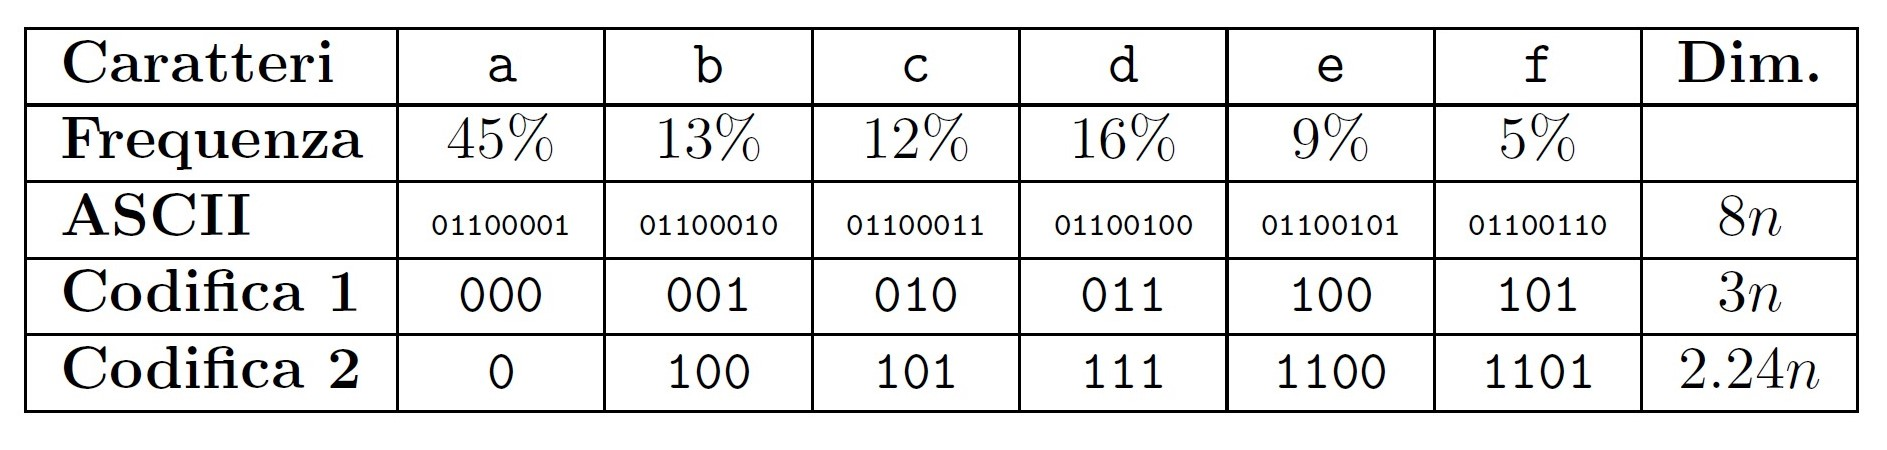
\includegraphics[width=0.8\textwidth]{../img/Greedy_1.jpg}
\caption{Possibili codifiche dei caratteri}
\end{figure} \\
Nella seguente immagine viengono mostrate codifiche differenti: ASCII, una basata sui caratteri effettivamente presenti all'interno del testo mentre l'ultima basata sulla frequenza con cui compaiono i caratteri. L'ultimo caso è il più interessante poichè utilizza meno bit per memorizzare il carattere che compare più di frequente: questo viene definito \textcolor{red}{codice a prefissi}.\\
In un codice a prefisso, \textcolor{red}{nessun codice è un profisso di un altro codice}. Ad esempio non è possibile mappare $a = 0$, $b = 1$, $c = 11$ poichè come interpreto poi 111111?
\newpage
\begin{flushleft}
\textbf{Rappresentazione ad albero per la decodifica}
\end{flushleft}
Un \textcolor{red}{albero binario di decodifica} viene così rappresentato
\begin{itemize}
	\item L'arco del figlio sinistro di ogni nodo è uno 0
	\item L'arco del figlio destro di ogni nodo è un 1
	\item Le sue foglie sono caratteri dell'alfabeto
\end{itemize}
\begin{figure}[h]
	\centering
	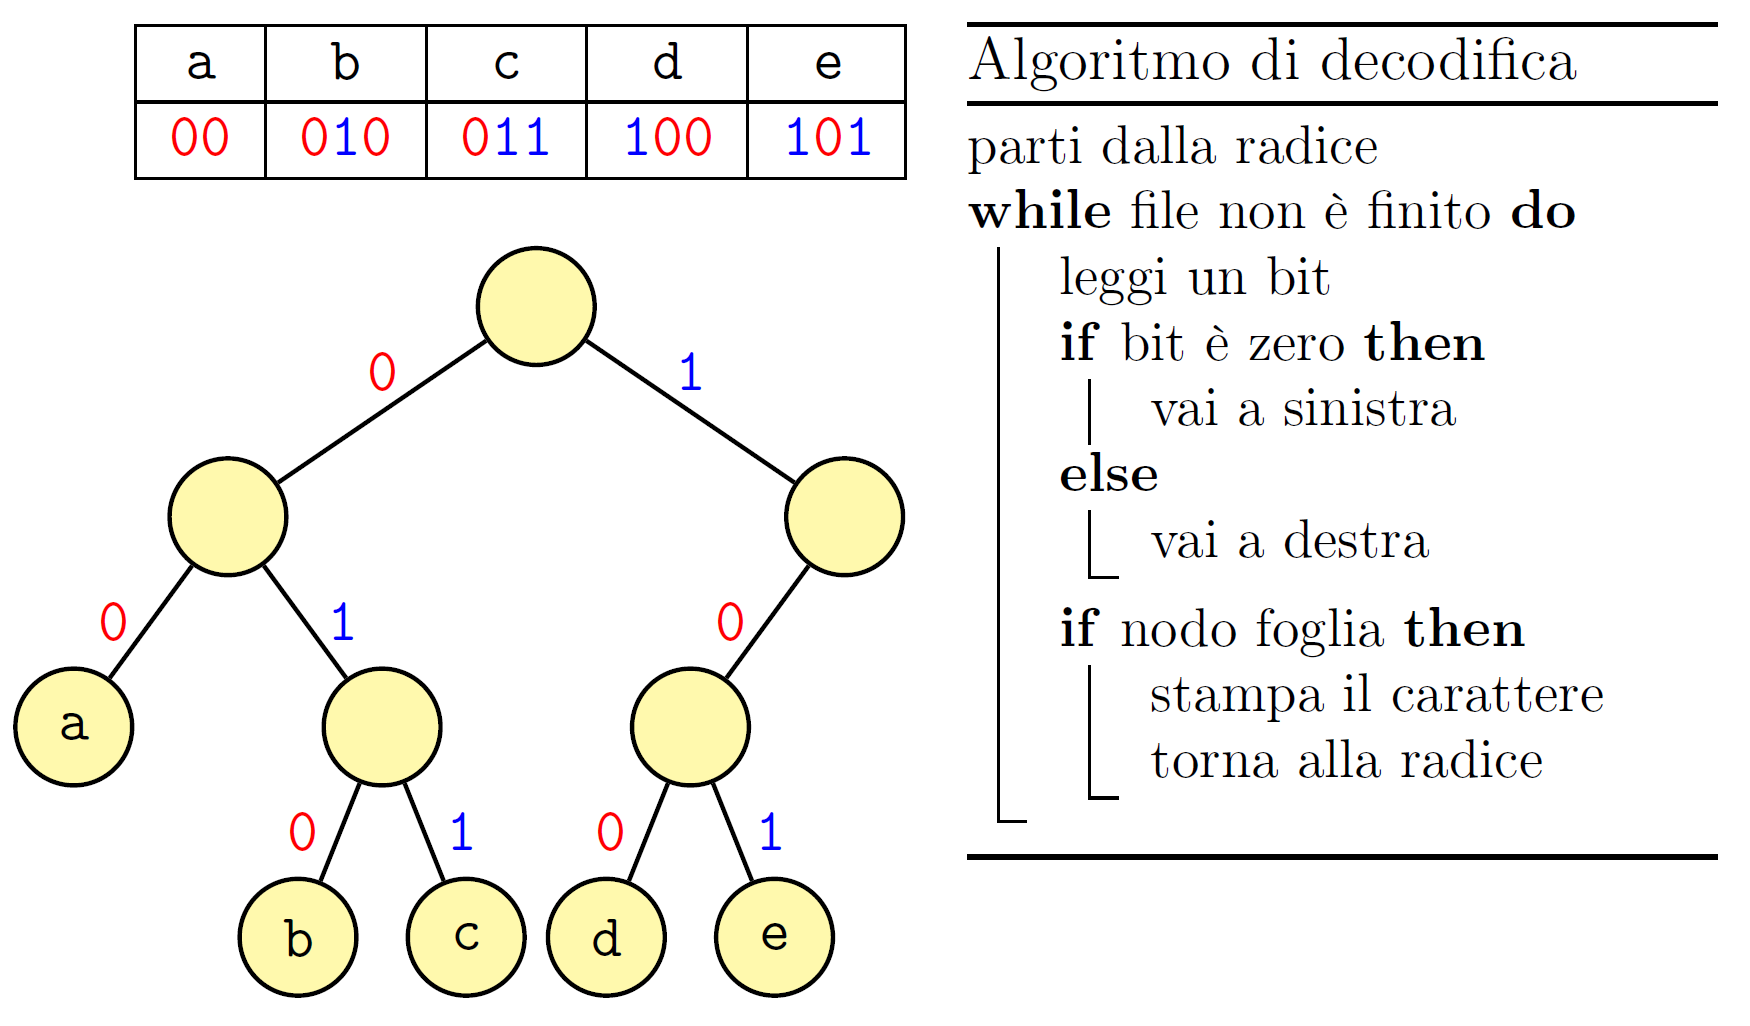
\includegraphics[width=0.7\textwidth]{../img/Greedy_2.png}
	\caption{Albero Binario di Decodifica - Rappresentazione}
\end{figure}
L'immagine precedente rappresenta un albero binario di decodifica che tuttavia ha un problema: il suo figlio destro infatti non serve a discriminare un carattere in particolare e quindi può essere tranquillamente tolto senza rendere la sequenza incomprensibile come nell'esempio precedente. Se quindi un nodo possiede un solo figlio all'interno di un albero binario di decodifica è possibile rimuovere il nodo e compattare l'albero.\\
\begin{figure}[h]
\centering
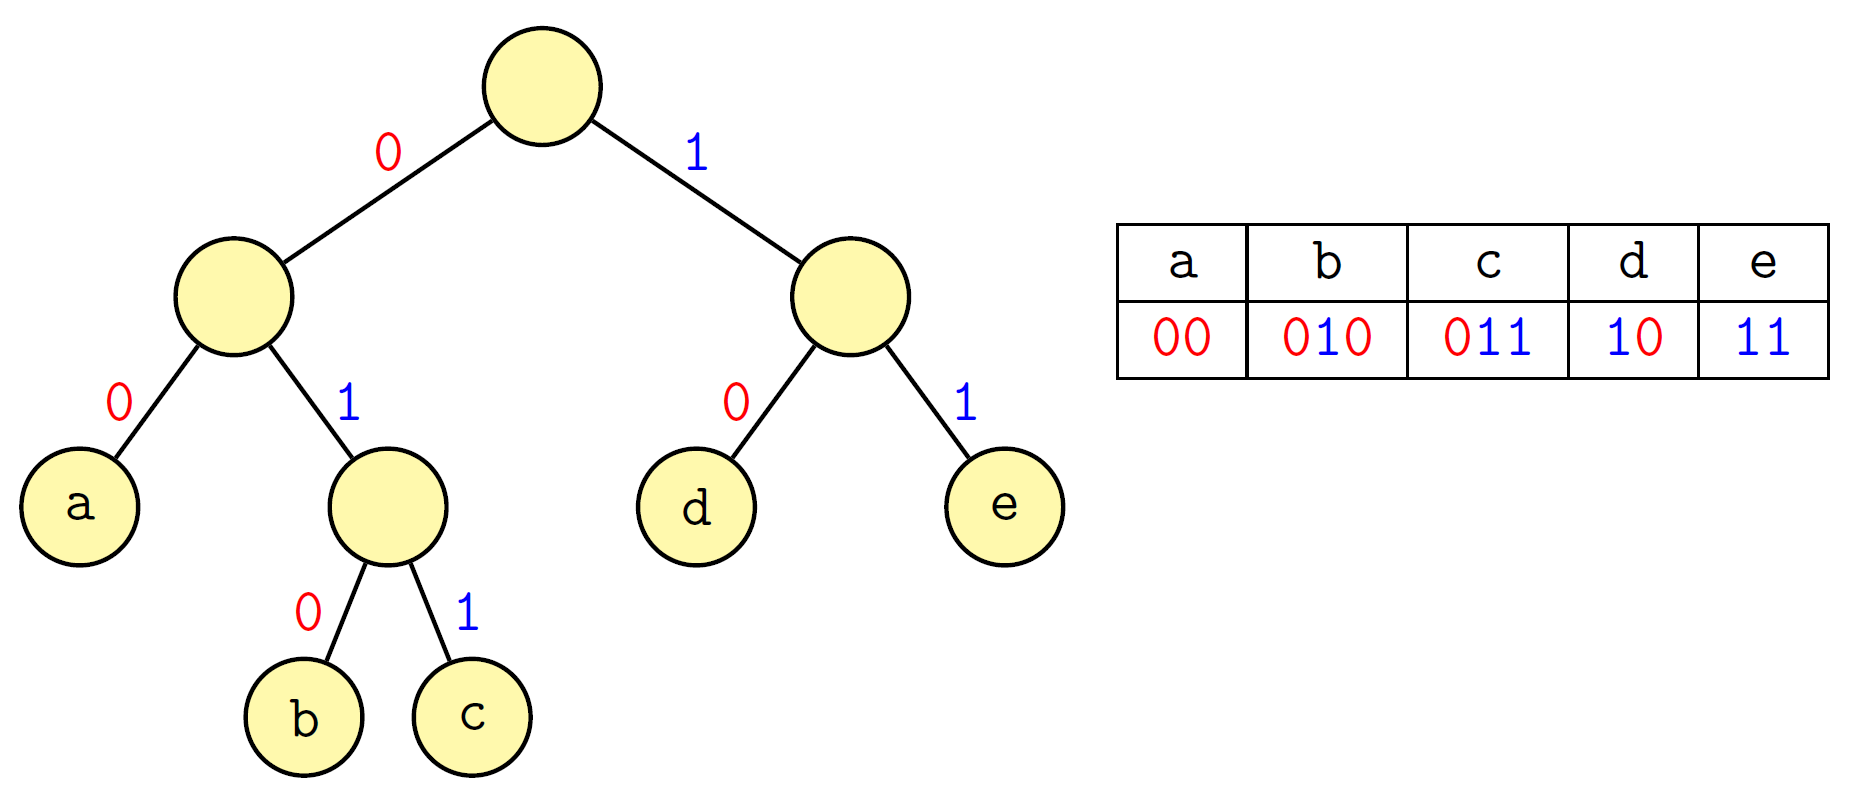
\includegraphics[width=0.7\textwidth]{../img/Greedy_3.png}
\caption{Albero Binario di Decodifica - Rimozione nodo}
\end{figure}
\newpage
\begin{flushleft}
\textbf{Definizione Formale del problema}
\end{flushleft}
Dato in input un file $F$ composto da caratteri nell'alfabeto $\mathcal{A}$, \textcolor{red}{quanti bit sono richiesti per codificare il file}?\\
Sia $T$ un albero che rappresenta la codifica e per ogni $c \in \mathcal{A}$ (carattere dell'alfabeto) sia $d_{T}(c)$ la profondità della foglia che rappresenta $c$. Dagli schemi precenti sappiamo che il codice per rappresentare $c$ richiederà allora $d_{T}(c)$ bit. Se $f[c]$ è il numero di occorrenze di $c$ in $F$, allora la dimenisone della codifica è
\begin{center}
	$C[F, T] = \sum_{c \in \mathcal{A}} f[c] \cdot d_{T}(c)$
\end{center}
Il principio del \textbf{Codice di Huffman} è quello di minimizzare la lunghezza dei caratteri che compaiono più frequentemente assegnando di conseguenza ai caratteri con minore frequenza i percorsi più lunghi all'interno dell'albero. Ogni codice è progettato per un file specifico
\begin{itemize}
	\item Si ottiene la frequenza dei caratteri
	\item Si costruisce il codice
	\item Si rappresenta il file tramite il codice
	\item Si aggiunge al file una rappresentazione del codice, per la decodifica
\end{itemize}
\textbf{Funzionamento dell'algoritmo}
\begin{enumerate}
	\item Costruisci una lista ordinata di nodi foglia per ogni carattere in base alla loro frequenza
	\item Rimuovi i due nodi con frequenza minore $f_{x}$ e $f_{y}$
	\item Crea un nodo padre con etichetta - e frequenza $f_{x} + f_{y}$
	\item Collega i due nuovi rimossi con il nuovo nodo
	\item Aggiungi il nodo creato alla lista 
	\item Se la lista ha un solo elemento termina altrimenti ripeti da 2
\end{enumerate}
\begin{lstlisting}[caption=creazione albero binario di decodifica]
TREE huffman(int[] c, int f, int n)
	for i = 1 to n do
		% Creo i nodi dell'albero contenenti i caratteri
		Q.insert(f[i], Tree(f[i], c[i])
	% Fino a quando non ho un solo nodo
	for i = 1 to n - 1 do
		% Seleziono dalla lista i nodi con minore frequenza
		$z_{1}$ = Q.deleteMin()
		$z_{2}$ = Q.deleteMin()
		% Creo un nuovo nodo che ha come foglie i due nodi estratti
		$z$ = Tree($z_{1}$.f + $z_{2}$.f, nil)
		$z$.left = $z_{1}$
		$z$.right = $z_{2}$
		% Inserisco il nodo creato nella lista
		Q.insert($z$.f, $z$)
	return Q.deleteMin()
\end{lstlisting}
\subsection{Alberi di Copertura di peso minimo}
Dato un grafo pesato, determinare come interconnettere tutti i suoi nodi minimizzando il costo del peso associato ai suoi archi.
\begin{itemize}
	\item \textcolor{red}{Albero di copertura (di peso) minimo}
	\item \textcolor{red}{Albero di connessione (di peso) minimo}
	\item \textcolor{red}{Minimum spanning tree}
\end{itemize}
\textbf{Definizione del problema}\\
Viene dato in input un grafo \textcolor{red}{$G = (V, E)$} non orientato e connesso e  \textcolor{red}{$w: V \times V \rightarrow \mathbb{R}$} funzione di peso (costo di connessione) t.c. se $[u, v] \in E$, allora $w(u, v)$ è il peso dell'arco $[u, v]$, altrimenti $+\infty$. Poichè $G$ è \emph{non orientato}, $w(u, v) = w(v, u)$.\\\\
\textbf{Albero di Copertura (Spanning Tree)}\\
Dato un grafo $G = (V, E)$ non orientato e connesso, un \textcolor{red}{albero di copertura} di $G$ è un sottografo $T = (V, E_{T})$ tale che 
\begin{itemize}
	\item $T$ è un albero
	\item $E_{T} \subseteq E$
	\item $T$ contiene tutti i vertici di $G$ \\
\end{itemize}
\textbf{Albero di Copertura di peso Vs Albero dei cammini minimi}
\begin{enumerate}
	\item Trovare l'albero di copertura il cui \textcolor{red}{peso totale} sia minimo rispetto a ogni altro albero di copertura, cioè per cui $w(T) = \sum_{[u, v] \in E_{T}}w(u, v)$ è minimo rispetto a tutti gli altri alberi di copertura
	\item Trovare l'albero di copertura con radice $v$ il cui \textcolor{red}{cammino da $v$ ad ogni altro vertice $u$} sia minimo
\end{enumerate}
\newpage
\end{document}
